\begin{frame}{Introduction}
	\vfill
	\begin{quotation}
		\centering
		Game theory is the mathematical study of interaction\\
		among independent, self-interested agents.\\
		{\color{colornote}-- Essentials of Game Theory, \cite{leyton2008essentials}}
	\end{quotation}

	\vfill
	\textbf{Examples}: economic and ecological games, machine learning, etc. \textcolor{colornote}{$\rightsquigarrow$ \emph{cybernetics}.}

	\vfill
	% ugh
	\onslide<2->{
		\alt<3>{
			Open games as a framework for compositional game theory

			\begin{center}
				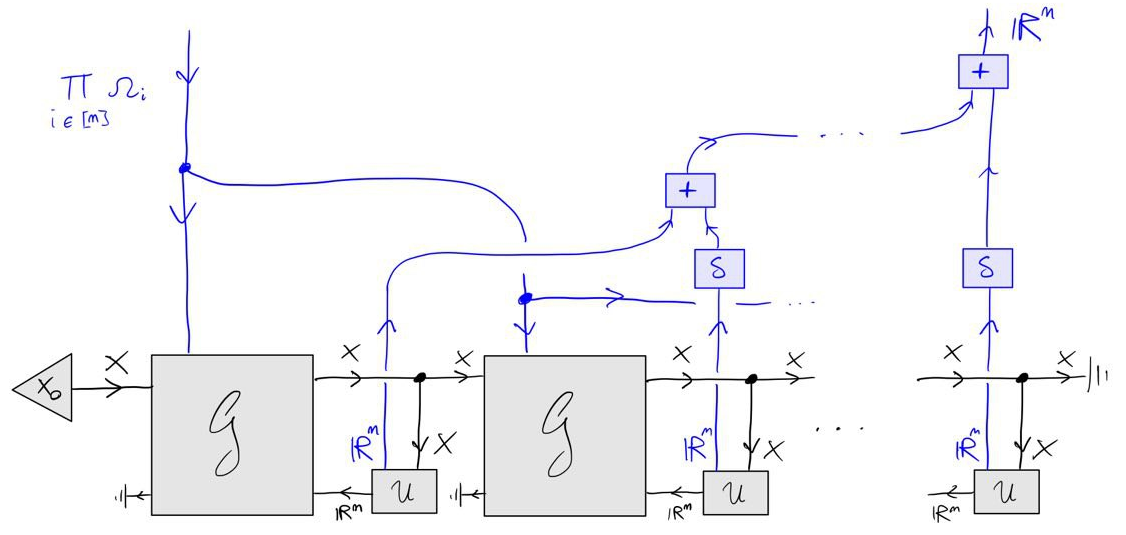
\includegraphics[width=.8\textwidth]{figures/og_ex.png}
			\end{center}

			Shows causality without being too unwieldy, compositional (\textcolor{coloraccent}{$\rightsquigarrow$ large scale}).\\
			Also: string diagrams are nice to work with!
		}{
			Classical game theory: \textbf{normal form} and \textbf{extensive form}

			\begin{center}
				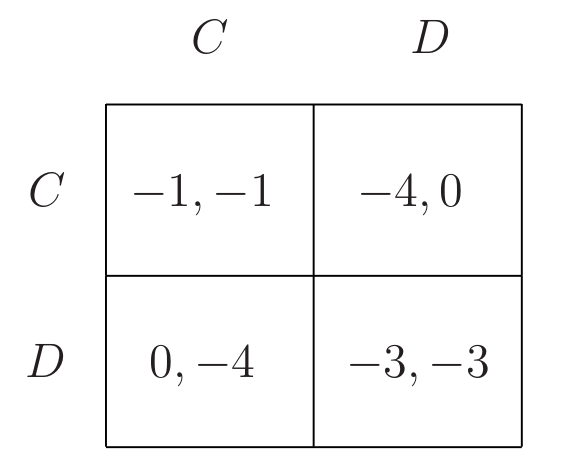
\includegraphics[width=.34\textwidth]{figures/pd_norm.png}
				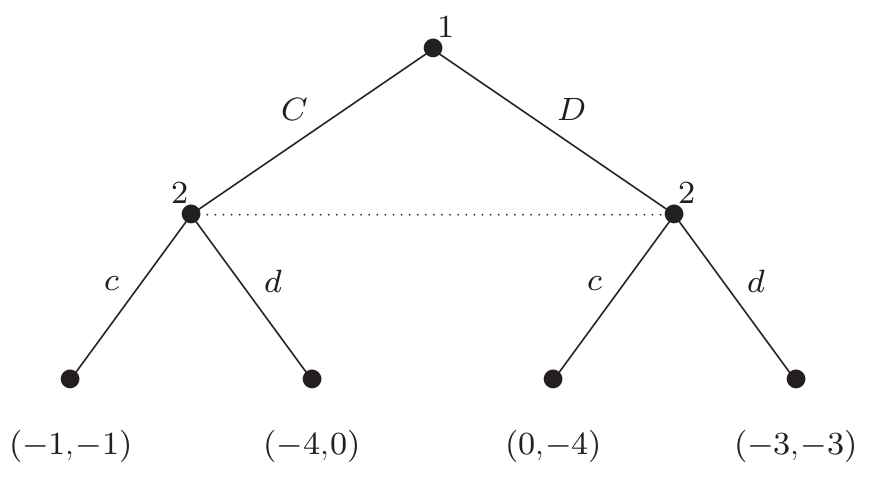
\includegraphics[width=.5\textwidth]{figures/pd_ext.png}
			\end{center}

			\textbf{Drawbacks}: too little information (NF), too much information (EF), unclear causal relationships (both). Most importantly: non-compositional! (\textcolor{coloraccent}{$\rightsquigarrow$ small scale})
		}
	}
\end{frame}

\begin{frame}{Introduction}
	\alt<2->{
		Translating EF to open games is non-trivial:
		\begin{enumerate}
			\item We need to seriously consider the problem of agency:
			\begin{enumerate}
				\item How do we represent correlated interests across a game?
				\item How do we represent player-dependent observational constraints (imperfect information)?
			\end{enumerate}
			\item We need operators to reflect the tree structure of the game.
		\end{enumerate}

		\onslide<3->{
			To do so, we introduce:

			\begin{enumerate}
				\item \textbf{Open games with agency}, an improved compositional (and conceptual) framework for games,
				drawing from/inspiring `open cybernetic systems'\footnote[frame]{\cite{capucci2021towards}}.
				\item An operator calculus for games, in particular new \textbf{choice operators}.
				%\item \textbf{Inductive data types for EF trees} with (im)perfect information.
			\end{enumerate}
		}
	}{
		Translating NF to open games is 'trivial' (there's only a utility function)...

		\begin{center}
			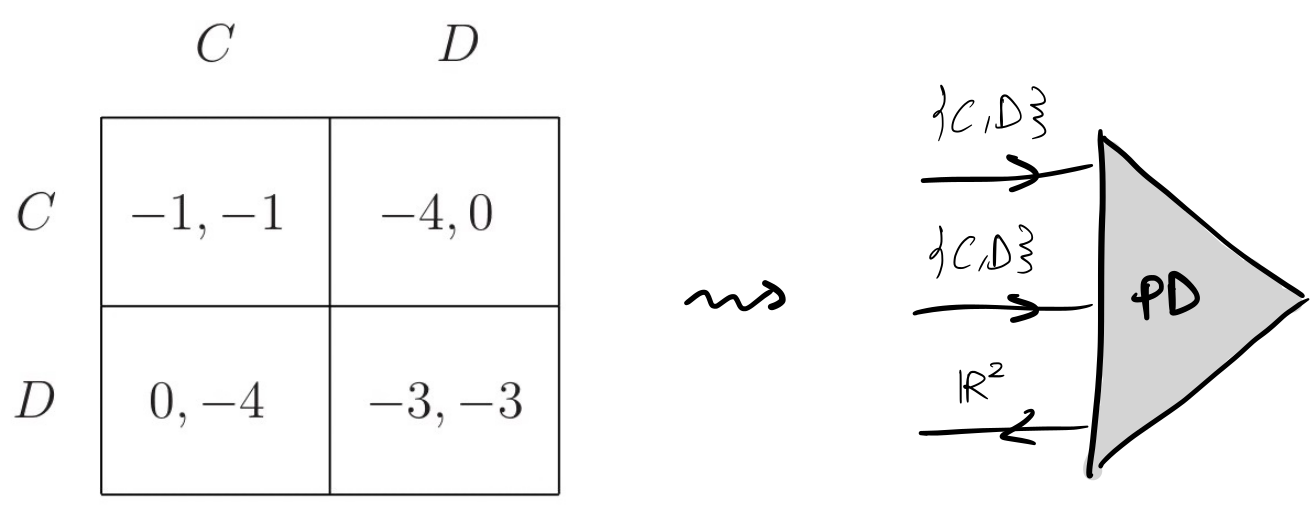
\includegraphics[width=.7\textwidth]{figures/nf_to_og.png}
		\end{center}
	}
\end{frame}

